\chapter{Agenti Razionali e Architetture}

\section{Credenze, Desideri e Intenzioni}

\dfn{Sistema Intenzionale}{
  Un sistema intenzionale è un sistema il cui comportamento può essere previsto dal metodo di attribuzione di credenze, di desideri e di acume razionale.
}

\nt{Per McCarthy, in alcuni casi si possono attribuire posizioni intenzionali a sistemi informatici.}

\clm{}{}{
  \begin{itemize}
    \item Più si sa di un sistema meno si fa affidamento a spiegazioni animistiche. 
    \item Con sistemi complessi una spiegazione meccanica potrebbe non essere praticabile.
  \end{itemize}
}

\dfn{Intenzioni e Astrazioni}{
  Più i sistemi di calcolo diventano complessi più si ha bisogno di astrazioni e metafore per spiegare il loro funzionamento. Le posizioni intenzionali sono una tale astrazione.
}

\nt{Le nozioni intenzionali sono quindi astrazioni che forniscono un modo semplice e familiare per descrivere, spiegare e prevedere il comportamento di sistemi complessi.}

\paragraph{I più importanti sviluppi sono basati su astrazioni:}

\begin{itemize}
  \item Procedure e funzioni. 
  \item Tipi di dati astratti (bloat). 
    \item Oggetti. 
    \item Agenti intelligenti e sistemi intenzionali. 
\end{itemize}

\subsection{Ragionamento su Azioni}

\dfn{Pratical Reasoning}{
  Il pratical reasoning è il ragionamento sulle azioni, sul processo di capire cosa fare.
}

\nt{Si distingue da theoretical reasoning che riguarda le credenze.}

\paragraph{Il pratical reasoning consiste in:}

\begin{itemize}
  \item \fancyglitter{Deliberazione}: decidere quale stato di cose vogliamo raggiungere. 
  \item \fancyglitter{Pianificazione} (menas-ends reasoning/planning): decidere come raggiungere questi stati di cose.
\end{itemize}

\nt{Dopo aver ottenuto un piano un agente tenterà di eseguirlo.}

\clm{}{}{
  \begin{itemize}
    \item Il calcolo è una risorsa preziosa per gli agenti, un agente deve controllare il suo ragionamento. 
    \item Gli agenti non possono deliberare a tempo indeterminato, a un certo punto devono smettere di deliberare e, dopo aver scelto uno stato di cose, impegnarsi per raggiungerlo.
  \end{itemize}
}

\cor{Intenzioni}{
  Ci riferiamo allo stato di cose che un agente ha scelto e al quale si impegna come le sue intenzioni.
}

\nt{Il ruolo delle intenzioni è quello di \fancyglitter{favorire la proattività}, ossia portare all'azione.}

\paragraph{Conseguenze:}

\begin{itemize}
  \item Persistenza delle azioni: se si adotta un'intenzione allora si deve insistere su essa e tentare di realizzarla. Se la motivazione cessa di esistere è razionale abbandore l'intenzione. 
  \item Le intenzioni vincolano il futuro pratical reasoning.
\end{itemize}

\paragraph{Intenzioni nel pratical reasoning:}

\begin{enumerate}
  \item Ci si aspetta che gli agenti trovino i modi per realizzare le loro intenzioni. 
  \item Le intenzioni forniscono un \fancyglitter{filtro} per l'adozione di altre intenzioni, che non devono entrare in conflitto. 
  \item Gli agenti monitorano il successo delle loro intenzioni e sono inclini a \fancyglitter{riprovare} se i loro tentativi falliscono. 
  \item  Gli agenti credono che le loro intenzioni siano possibili\footnote{Gli agenti sono come Naruto che vuole diventare Hokage.}. 
  \item Gli agenti non credono che non realizzeranno le loro intenzioni\footnote{Gli agenti sono come Naruto che vuole diventare Hokage pt. 2.}. 
  \item Nelle giuste circostanze gli agenti credono che realizzeranno le loro intenzioni. 
  \item Gli agenti non devono necessariamente avere intenzioni su tutti gli effetti collaterali delle loro intenzioni.
\end{enumerate}

\clm{}{}{
\begin{itemize}
  \item Il problema di avere l'intenzione di realizzare qualcosa credendo che non sia possibile è noto come \fancyglitter{intention-belief inconsistency} e non è razionale. (punto 5)
  \item Il problema di avere l'intenzione di realizzare qualcosa senza credere che la realizzeranno è noto come \fancyglitter{intention-belief incompleteness} ed è una proprietà accettabile per gli agenti razionali. (punto 6)
  \item Il problema al punto 7 è noto come \fancyglitter{package deal}. 
  \end{itemize}
}

\subsection{Modellazione Logica di Agenti BDI}

\begin{itemize}
  \item La logica riguarda principalmente il \fancyglitter{rational balance} relativo a beliefs, goals, plans, intentions, commitments e azioni di agenti autonomi. 
  \item L'obiettivo principale è di esplorare le reazioni che le intenzioni hanno nel mantenere questo bilanciamento. 
  \item Questo deve essere analizzato con \fancyglitter{beliefs}, \fancyglitter{desires} e \fancyglitter{intentions} (BDI).
\end{itemize}

\paragraph{La logica di Cohen e Levesque ha 4 operatori modali principali:}

\begin{itemize}
  \item $(BEL\: i\: \phi)$: l'agente $i$ crede $\phi$.
  \item $(GOAL\: i\: \phi)$: l'agente $i$ ha il goal (desire) $\phi$. 
  \item $(HAPPENS\:\alpha)$: l'azione $\alpha$ occorre al passo successivo. 
  \item $(DONE\: \alpha)$ l'azione $\alpha$ è appena occorsa.
\end{itemize}

\nt{Un'azione $\alpha$ può essere un evento primitivo oppure complesso. L'intenzione non è un operatore primitivo, ma può essere derivato.}

\paragraph{Successivamente viene proposta un'altra logica, da Rao e Georgeff (BDI):}

\begin{itemize}
  \item Ci sono tre modalità: $BEL$, $GOAL$ e $INTEND$. 
  \item I mondi sono strutture temporali branching time. 
\end{itemize}

\paragraph{È possibile descrivere commitments diversi:}

\begin{itemize}
  \item Agente \fancyglitter{blindy committed} (fanatical): mantiene le sue intenzioni finché non arriva a credere di averle soddisfatte. $$INTEND(AF\:\phi) \Rightarrow A(INTEND(AF\:\phi) \cup BEL(\phi))$$
  \item Agente \fancyglitter{Single-minded committed}: mantiene le sue intenzioni finché crede che queste possano essere realizzabili.  $$INTEND(AF\:\phi) \Rightarrow A(INTEND(AF\:\phi) \cup (BEL(\phi) \lor \neg BEL(EF\:\phi)))$$
  \item Agente \fancyglitter{open-minded}: mantiene le sue intenzioni finché queste intenzioni sono ancora i suoi goals. $$INTEND(AF\:\phi) \Rightarrow A(INTEND(AF\:\phi) \cup (BEL(\phi) \lor \neg GOAL(EF\:\phi)))$$
\end{itemize}
\pagebreak
\subsection{Un'Architettura per agenti BDI}

\begin{figure}[!h]
    \centering
    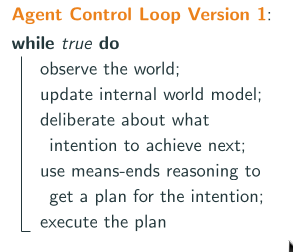
\includegraphics[scale=0.65]{03/agent1.png}
    \caption{Una prima versione di un agente che utilizza il pratical reasoning.}
\end{figure}

\paragraph{Nella prima versione:}

\begin{itemize}
  \item I processi di deliberation e means-end reasoning non sono immediati, hanno un costo nel tempo.
  \item Supponiamo che l'agente inizi a deliberare all'istante $t_0$, inizi il means-end reasoning all'istante $t_1$ e che cominci l'esecuzione del piano all'istante $t_2$: 
    \begin{itemize}
      \item Il tempo per deliberare è $t_d= t_1 - t_0$. 
    \item Il tempo per il means-end reasoning è $t_{me} = t_2 - t_1$. 
    \item Supponiamo inoltre che la deliberazione sia ottimale, cioè se si seleziona un'intenzione da raggiungere essa sia la migliore per l'agente. 
    \item Al tempo $t_1$ l'agente ha selezionato l'intenzione da raggiungere che sarebbe stata ottimale se fosse stata raggiunta all'istante $t_0$.
      \item A meno che $t_d$ sia molto piccolo c'è il rischio che l'intenzione non sia più ottimale (calculative rationality). 
    \end{itemize}
\end{itemize}

\paragraph{L'agente avrà un comportamento complessivo ottimale nelle seguenti circostanze:}

\begin{itemize}
  \item Quando il tempo impiegato per i processi di deliberazione di means-end è estremamente piccolo. 
  \item Quando il mondo è \fancyglitter{statico} mentre l'agente effettua o suoi processi. 
  \item Quando un'intenzione ottimale se raggiunta al tempo $t_0$ (il momento in cui si osserva il mondo) è garantita rimanere ottimale fino al tempo $t_2$ (il tempo in cui l'agente ha determinato le azioni per raggiungere le intenzioni).
\end{itemize}

\begin{figure}[!h]
    \centering
    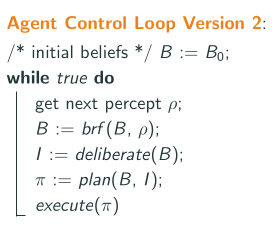
\includegraphics[scale=0.65]{03/agent2.png}
    \caption{Seconda versione di un agente che utilizza il pratical reasoning.}
\end{figure}

\paragraph{Nella seconda versione:}

\begin{itemize}
  \item $B$: credenze. 
  \item $I$: intenzioni. 
  \item $brf()$: revisione delle credenze. 
  \item $deliberate()$: deliberazione delle intenzioni. 
  \item $plan()$: pianificazione.
  \item La pianificazione è la progettazione di una sequenza di azioni che consentirà di raggiungere l'obiettivo desiderato. 
  \item Dati: 
    \begin{itemize}
      \item Una rappresentazione dell'obiettivo/intenzione da raggiungere. 
      \item Una rappresentazione delle azioni che può eseguire. 
      \item Una rappresentazione dell'ambiente.
    \end{itemize}
  \item Si tratta di automatica programming.
\end{itemize}

\qs{}{Come un agente delibera?}

\begin{itemize}
  \item \fancyglitter{Option generation}: inizia cercando di capire quali sono le opzioni a sua disposizione sulla base delle proprie informazioni e credenze. 
  \item \fancyglitter{Filtering:} sceglie tra le opzioni possibili e si impegna verso di esse. 
\end{itemize}

\nt{Le opzioni scelte sono le intenzioni.}

\begin{figure}[!h]
    \centering
    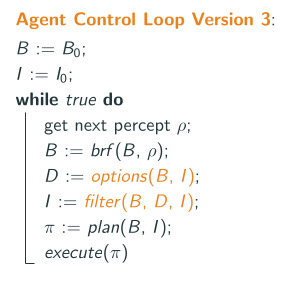
\includegraphics[scale=0.65]{03/agent3.png}
  \caption{Terza versione di un agente che utilizza il pratical reasoning.}
\end{figure}

\paragraph{Nella terza versione:}

\begin{itemize}
  \item $option()$: l'agente genera un insieme di possibili alternative. Rappresenta la generazione di opzioni tramite una funzione. 
  \item $filter()$: l'agente sceglie tra le alternative che competono e si impegna a raggiungerle. 
  \item Quando un'opzione è restituita da filter diciamo che l'agente ha fatto un \fancyglitter{commitment} verso tale opzione. 
  \item Il commitment implica persistenza temporale, per cui un'intenzione adottata non dovrebbe essere immediatamente abbandonata.
\end{itemize}

\dfn{Commitment Strategies}{
  Il meccanismo che un agente usa per determinare quando e come un'intenzione possa essere abbandonata.
}

\nt{I tipi di strategie sono gli stessi dei tipi di agente (blind, single-minded, open-minded).}

\begin{figure}[!h]
    \centering
    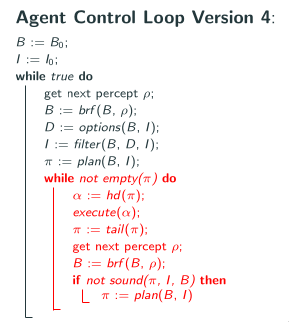
\includegraphics[scale=0.65]{03/agent4.png}
  \caption{Quarta versione di un agente che utilizza il pratical reasoning.}
\end{figure}

\paragraph{Nella quarta versione:}

\begin{itemize}
  \item Si ripianifica se qualcosa va storto. 
  \item È ancora presente overcommitment rispetto alle intenzioni: non si ferma a valutare se le sue intenzioni siano più o meno adeguate (blind). 
\end{itemize}
\pagebreak
\begin{figure}[!h]
    \centering
    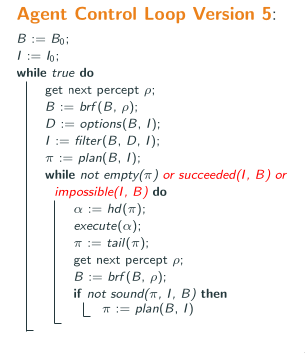
\includegraphics[scale=0.65]{03/agent5.png}
  \caption{Quinta versione di un agente che utilizza il pratical reasoning.}
\end{figure}

\paragraph{Nella quinta versione:}

\begin{itemize}
  \item Ci si ferma per determinare se le intenzioni hanno avuto successo o se sono diventate impossibili da soddisfare (single-minded). 
  \item L'agente può riconsiderare le sue intenzioni ogni volta che il controllo è sul ciclo esterno, ossia quando:
    \begin{itemize}
      \item Ha completamente eseguito un piano per raggiungere le sue intenzioni correnti. 
      \item Ritiene di aver raggiunto le sue attuali intenzioni.
      \item Crede che le sue attuali intenzioni non siano più possibili.
    \end{itemize}
  \item Questo limita il modo in cui consente a un agente di riconsiderare le sue intenzioni.
\end{itemize}
\pagebreak
\begin{figure}[!h]
    \centering
    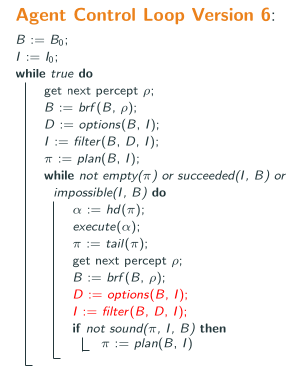
\includegraphics[scale=0.65]{03/agent6.png}
  \caption{Sesta versione di un agente che utilizza il pratical reasoning.}
\end{figure}

\paragraph{Nella sesta versione:}

\begin{itemize}
  \item Riconsidera le intenzioni dopo l'esecuzione di ogni azione (open-minded).
  \item Tuttavia la riconsiderazione delle intenzioni costa: 
    \begin{itemize}
      \item Un agente che non si ferma abbastanza spesso continuerà a tentare di raggiungere le sue intenzioni anche dopo che sarà chiaroo che non possono essere raggiunte. 
      \item Un agente che riconsidera costantemente dedica poco tempo a raggiungere le sue intenzioni.
    \end{itemize}
\end{itemize}

\begin{figure}[!h]
    \centering
    
\includegraphics[scale=0.35]{03/shinji.png}
  \caption{L'agente che riconsidera costantemente be like.}
\end{figure}

\pagebreak
\subsection{Riconsiderazione delle Intenzioni}

\begin{figure}[!h]
    \centering
    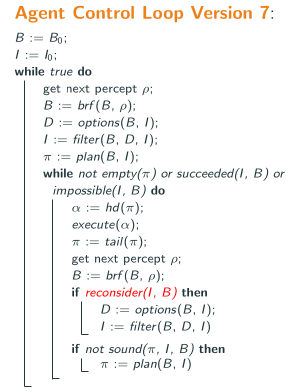
\includegraphics[scale=0.65]{03/agent7.png}
  \caption{Settima versione di un agente che utilizza il pratical reasoning.}
\end{figure}

\paragraph{Nella settima versione:}

\begin{itemize}
  \item Incorpora una componente di controllo esplicita \fancyglitter{meta-livello} che decide se eseguire o meno la riconsiderazione. 
\end{itemize}

\begin{figure}[!h]
    \centering
    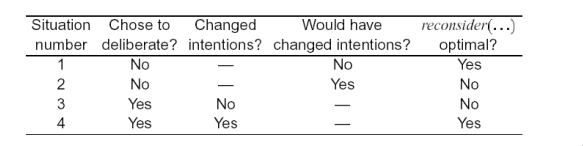
\includegraphics[scale=0.7]{03/controllo.png}
  \caption{Componente meta-livello.}
\end{figure}

\nt{Il problema è che la reconsider() è una funzione oracolo, per cui va implementata mediante euristiche e studi specifici sul dominio. Il costo di questa funzione dovrebbe essere molto inferiore al costo del processo deliberativo stesso.}

\paragraph{Kinny e Georgeff hanno investigato ciò in maniera sperimentale:}

\begin{itemize}
  \item Due tipi di agenti: 
    \begin{itemize}
      \item \fancyglitter{Bold agents}: non si fermano mai a riconsiderare le intenzioni. 
      \item \fancyglitter{Cautious agents}: riconsiderano le intenzioni dopo ogni azione.
    \end{itemize}
  \item Considerazioni:
    \begin{itemize}
      \item Se l'ambiente non cambia rapidamente gli agenti bold funzionano meglio. 
      \item Se l'ambiente cambia costantemente gli agenti cautious funzionano meglio.
    \end{itemize}
\end{itemize}





